%! Author = oskin
%! Date = 21.08.2023

% Preamble
\documentclass[11pt]{article}

% Packages
\usepackage{amsmath}
\usepackage{csquotes}
\usepackage{hyperref}
\usepackage{graphicx}
\graphicspath{ {./assets/} }

\title{Spectrum Bloom: A self-developing, sustainable, eUTxO-native framework for decentralized finance}
\author{Ilya Oskin \\ \href{mailto:i.oskin@spectrumlabs.fi}{i.oskin@spectrumlabs.fi}}
\date{Aug 2023}

% Document
\begin{document}

    \begin{sloppypar}
        \maketitle


        \begin{abstract}
            Over the past few years eUTxO blockchains such as Ergo and Cardano have seen rapid development of decentralized exchanges (DEXes).
            Following the success of early EVM-based DEXes multiple projects building on top of novel eUTxO model, with ErgoDEX being the pioneer, managed to deliver quality protocols.
            However, all of these early attempts suffer from lack of transparency, composability and poor performance.
            In this work we make an attempt to analyze those weaknesses and address them in a new protocol based on principles of decentralization, openness, transparency and sustainability.
        \end{abstract}


        \section{Preliminaries}\label{sec:preliminaries}

        \subsection{DeFi primitives}\label{subsec:defi-primitives}
        Decentralized finance (DeFi) consists of heterogeneous modules, each implementing some financial tool as a small (or not so small) protocol.
        We refer to such modules as to \enquote{primitives}, supposing that they form an ecosystem and can potentially be composed.
        Some of these primitives are discussed below.

        \textbf{Automated Market Maker.} An integral part of the decentralized finance (DeFi) ecosystem, decentralized exchanges (DEXs) \
        with automated market maker (AMM) protocols~\cite{Xu_2023}.
        AMM uses mathematical models to set the price and match buyers and sellers rather than merely matching buy and sell orders, as in \
        traditional order-books.
        AMM is best in markets with low liquidity.
        One of the features of AMM is that liquidity providers add assets to the exchange for a fee, and the market benefits from an \
        increase in liquidity, smaller latency, limited price slippage, and less market volatility when using this additional liquidity.

        \textbf{Order Book.} A similar construction to the one widely used on centralized exchanges.
        Orders are waiting for other orders to be matched, or for a cancellation.
        There are the following two types of orders --~\enquote{buy} (i.e. buy base asset for quote),~\enquote{sell} (i.e. sell base asset for quote).
        Order-book DEX has the advantage of working best for those pairs with high liquidity.

        \textbf{Algorithmic Stablecoin.} An algorithmic stablecoin protocol that behaves like an autonomous bank that buys and sells stablecoins for a price in a range that is pegged to a target price~\cite{cryptoeprint:2021/1069}.

        \subsection{Scope of the work}\label{subsec:scope-of-the-work}
        In this work we analyze high level approach to designing decentralized exchange systems.
        Thus, we abstract away from concrete implementations of financial primitives like AMM, Order Book or Stablecoin Bank, \
        and will refer to them as to abstract \enquote{liquidity sources}.

        The primary goal of this work is to design a protocol applicable to any exchange type and interoperable with any DeFi primitive \
        instantiation by default with only one requirement: openness of the target primitive implementation.

        \subsection{System Model}\label{subsec:system-model}
        We assume a UTxO based blockchain that supports multi-stage contracts (extended-UTxO) ~\cite{chepurnoy2018selfreproducing} and multi-token functionality.
        In our model Decentralized Exchange (DEX) is a protocol that consists of two pillars:
        \begin{enumerate}
            \item \textbf{On-Chain}.
            On-Chain part is defined in terms of unspent transaction outputs (UTxOs) and validators guarding them.
            Therefore, state of the DEX is encoded solely in ledger.
            \item \textbf{Off-Chain}.
            A set of event handlers that, upon receiving of event, emit a transaction triggering state transition in on-chain part.
        \end{enumerate}

        \subsubsection{Liquidity pooling}
        We assume that in the context of eUTxO model all forms of liquidity pooling (e.g.\ AMM, Order Book, Stablecoin Bank etc.) are \
        represented as a single UTxO guarded with a specific validator script that assures all transactions applied to the pool are legitimate.

        \begin{figure}[h]
            \centering
            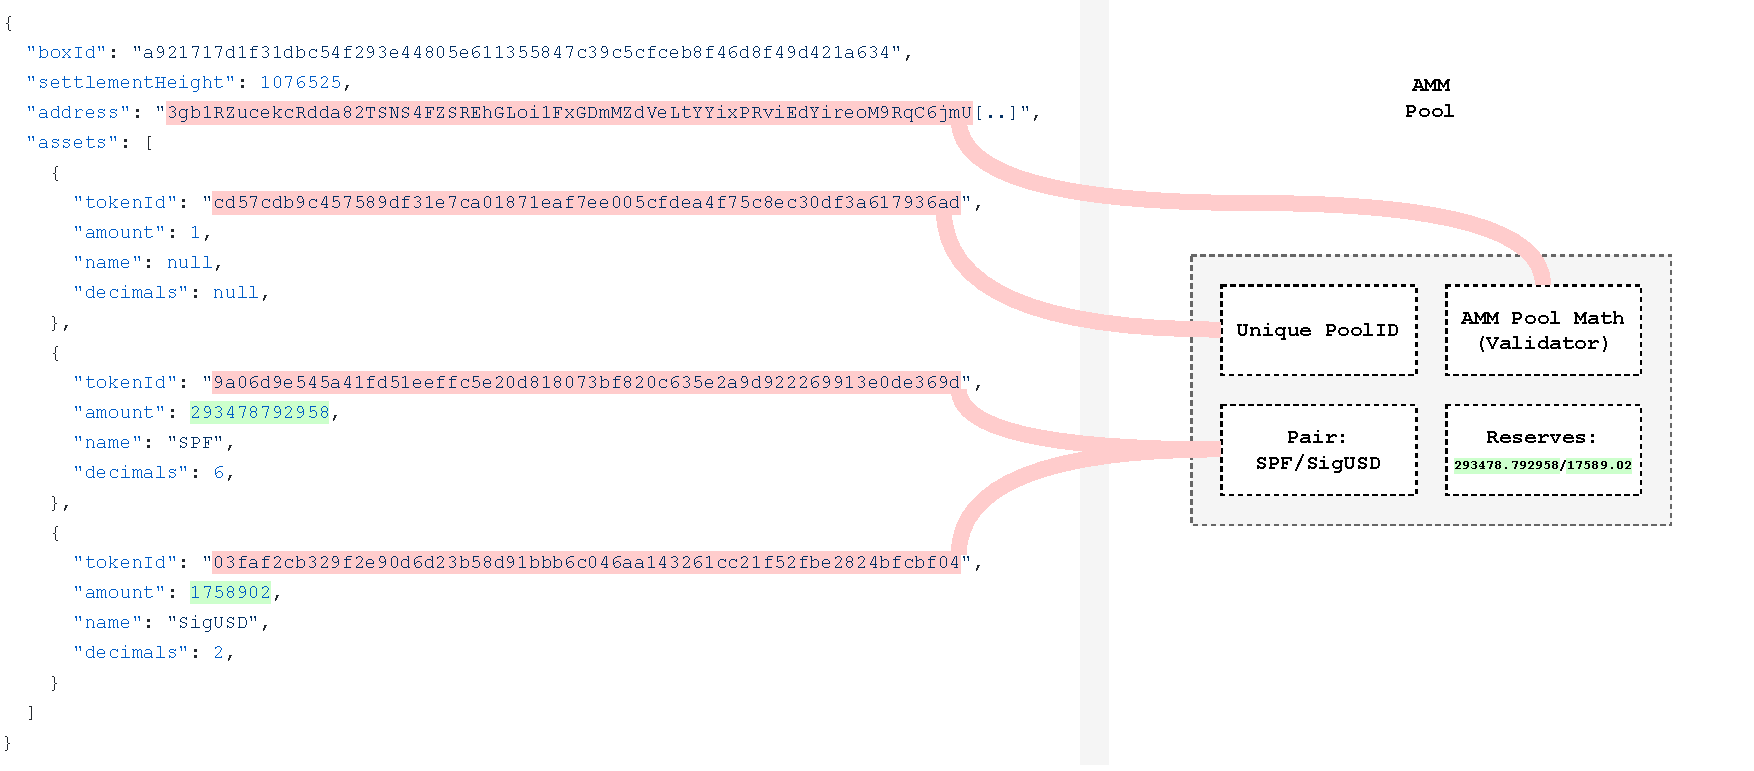
\includegraphics[width=0.96\textwidth]{amm-utxo}
            \caption{Illustration of a raw UTxO in Ergo~\cite{ergo2019wp} blockchain mapping to an AMM liqudity pool encoded into it.}
            \label{fig:figure}
        \end{figure}

        \subsection{Structure}\label{subsec:structure}
        The rest of the paper is structured as follows: in Section~\ref{sec:classical-dex-design} we first describe initial \enquote{classical} \
        approach to designing a DEX and discuss its weaknesses.
        Then in Section~\ref{sec:spectrum-framework} we iteratively address those weaknesses in a novel framework.
        Section~\ref{sec:autonomous-account} is dedicated to detailed explanation and extension of the \enquote{Autonomous Account} introduced \
        in Section~\ref{sec:spectrum-framework}.


        \section{Classical DEX design}\label{sec:classical-dex-design}
        eUTxO pioneers faced a challenge when first tried to port protocols such as Uniswap~\cite{uniswap2020evm}: \
        while EVM implementations allowed its users to transact with liquidity pools directly from clients, on eUTxO such scenario was extremely impractical.
        The root of the problem lays in the nature of eUTxO, unlike Account model it requires that all inputs of a transaction are deterministic.
        Therefore, direct transaction with shared, atomic on-chain entities like aggregated liquidity pool would result in race conditions \
        (on practice that means that only one order can succeed in a certain time window, others must be refunded and recreated).

        A classical approach to model a DEX protocol is to synchronize user access to a shared liquidity pool via on-chain orders which are \
        then picked up, ordered and executed by off-chain bots shortly after.
        On-chain order is encoded into a UTxO carrying some input value (e.g.\ some amount of base asset in case of limit sell order) \
        and guarded with a validator script that ensures that the order is executed at a fair price provided by concrete liquidity pool \
        at the time of actual order execution.
        Validator script guarding an order should contain concrete specification of a pool it is intended to be applied to, otherwise it won't \
        be able to read fair price from it.

        \begin{figure}[h]
            \centering
            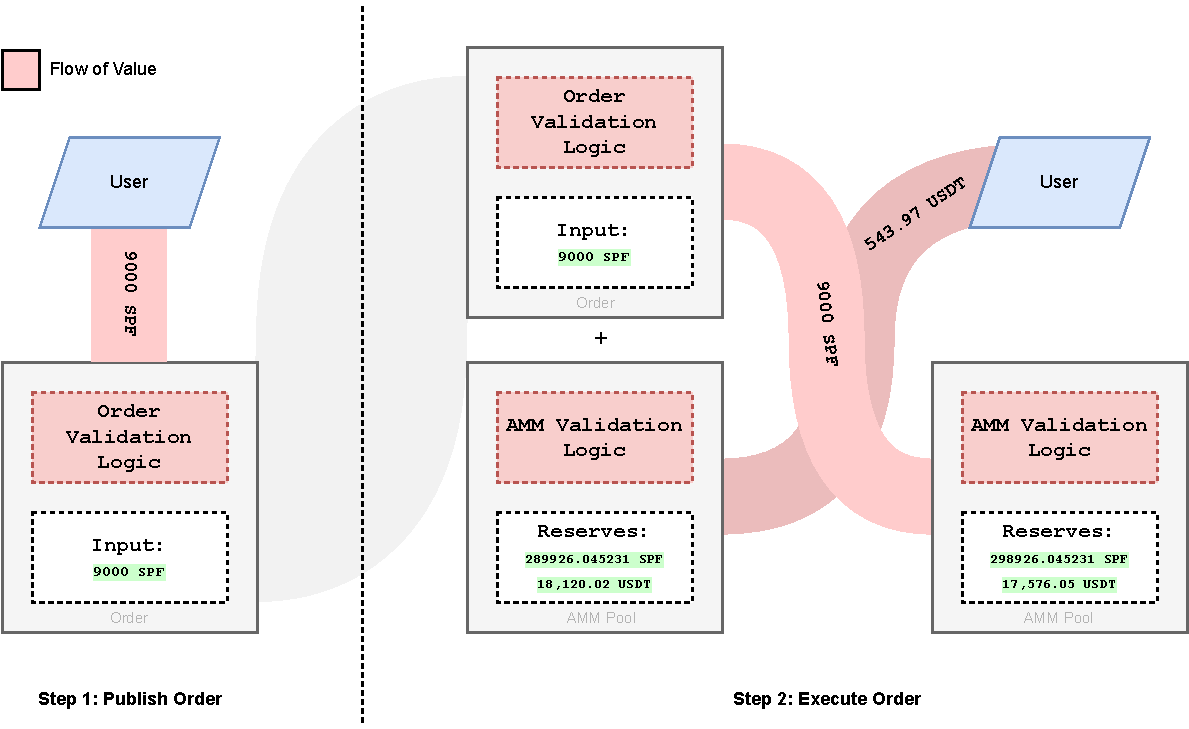
\includegraphics[width=0.96\textwidth]{pool+order}
            \caption{A diagram that shows how users interact with aggregated liquidity pools via orders.
            At first step a client publishes an order moving some of his funds into it, at the second step
            random off-chain operator matches this order with a proper pool and executes the deal.}
            \label{fig:figure2}
        \end{figure}

        \subsection{Limitations of classical design}\label{subsec:limitations-of-classical-design}
        \textbf{Lack of Transparency.} The need for off-chain execution creates a separate market with its own incentives for actors willing to serve the protocol.
        In the worst case there is a monopoly of project team exclusively having permission to do off-chain execution.
        Best practice currently is to allow permissionless off-chain execution.
        On the open market a number of agents compete to execute each order to earn execution fees, but not only that.
        Another way of taking profit from execution is to do what's called \enquote{Frontrunning} or \enquote{Blockchain Extractable Value}~\cite{bartoletti2023theoretical}.
        BEV allows to extract additional value from users, beyond what they are willing to pay as fees.
        Due to opaque nature of execution users neither know who will handle their order in the end, nor do they have any control over the execution.

        As a result lack of transparency leads to incentive model that does not always reward those actors who serve the protocol in the best way.

        \textbf{Inefficiency.} On-chain orders require an extra transaction.
        As a result user has to cover fees for both order publishing transaction and execution transaction.
        In the case of order execution failure (e.g.\ due to price slippage or expiration) an additional transaction is required to \
        redeem funds locked in the order.

        \textbf{Poor Composability.} Orders are specialized to work with concrete implementation of a liquidity pool to be able to \
        properly check correctness of execution.
        This renders it impossible to compose orders with different sources of liquidity (e.g.\ liquidity pools of the same pair on \
        different DEXes).


        \section{Spectrum Bloom Framework}\label{sec:spectrum-framework}
        We are now presenting a novel DEX framework by gradually improving the classical approach.

        \subsection{Explicit Order Routing}\label{subsec:making-execution-transparent}
        We modify classical construction in a way that off-chain executors are now required to register their public keys, those keys will serve as unique identifiers.
        Users are now able to explicitly specify the set of off-chain operators allowed to execute their orders.

        To implement this we append the following condition to the validator script: \
        $\exists PK_i: verify(\sigma, PK_i, H(T)) \wedge PK_i \in R$, \
        where $PK_i$ -- public key of $i-th$ executor, $verify(\sigma, PK, m) \rightarrow 0 | 1$ -- function that verifies signature $\sigma$ against public key $PK$ and message $m$, \
        $H(T)$ -- cryptographic hash of transaction, $R$ -- set of executors allowed to execute the order.

        With off-chain executors being publicly identifiable clients can now track their performance off-chain (e.g.\ detect MEV, measure response time, etc.) and \
        render rating tables to inform users.
        This way the profitability function of executors can be adjusted off-chain without the need to modify the protocol by simply \
        applying different rating functions on clients.

        \subsection{Green Orders}\label{subsec:off-chain-orders}
        We are now eliminating the need for on-chain orders by encoding them into a message that is relayed to the desired executors off-chain.
        We call such off-chain orders \enquote{green} because of their zero on-chain overhead.
        The structure of the message is described in Table~\ref{tab:table} below.

        \begin{table}[h]
            \begin{center}
                \begin{tabular}{ | r l | }
                    \hline
                    OrderBody = & $\text{OrderParams} \times \text{Nonce}$ \\
                    Message =   & $\text{OrderBody} \times \sigma$         \\
                    \hline
                \end{tabular}
            \end{center}
            \caption{Message structure. The user authorizes the order by signing its contents and attaching the proof $\sigma$.
            OrderParams -- parameters of the order, e.g. quote and base asset, price, etc., Nonce -- monotonically increasing counter to prevent replay attacks.}
            \label{tab:table}
        \end{table}

        In order to be able to actually execute off-chain orders some kind of on-chain entity that can validate execution and permit the \
        release of user (without the need to interact with user) funds is required.
        At this point we introduce Autonomous Account (AA) over eUTxO -- an on-chain entity that is able to read order message, validate execution, \
        and release the amount of user funds required to execute the deal.
        To work with AA the user has to deposit some funds that he is willing to trade into it.

        \begin{figure}[h]
            \centering
            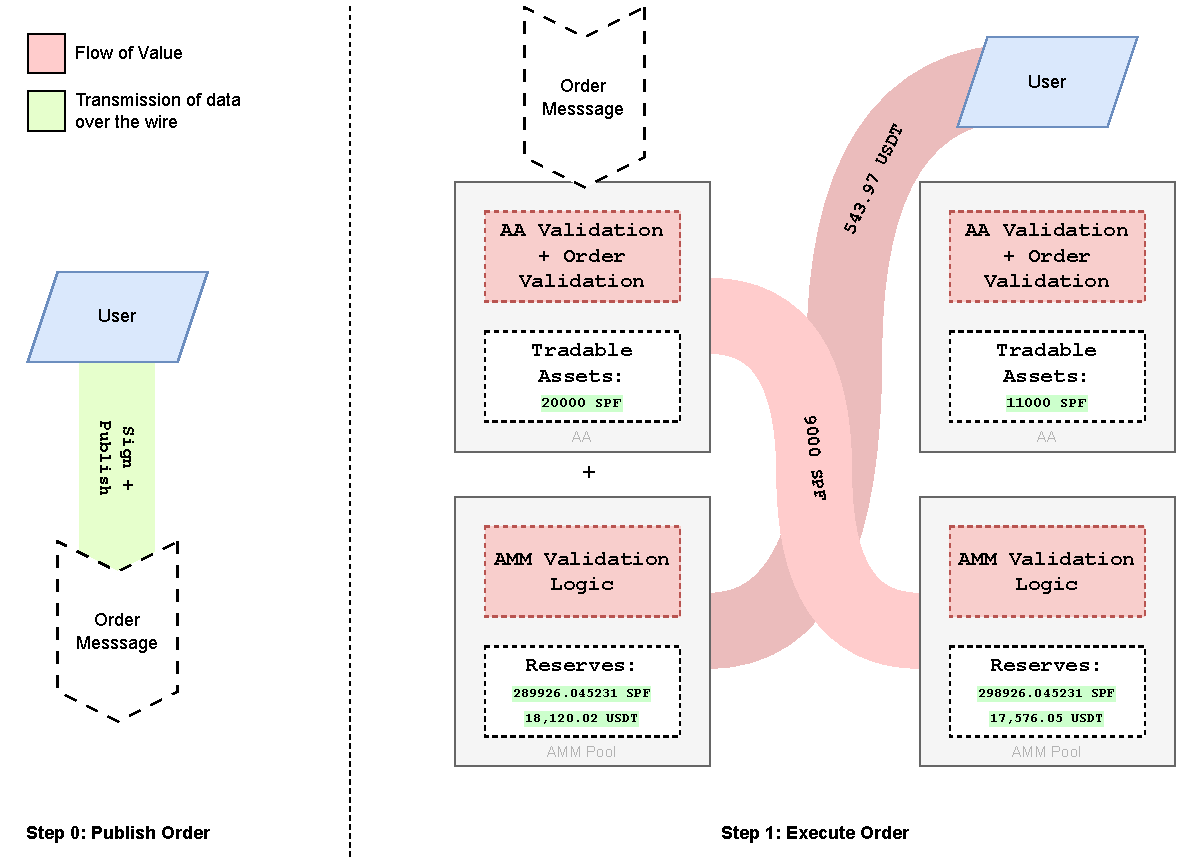
\includegraphics[width=0.96\textwidth]{pool+offchain_order}
            \caption{A modified construction. Step 0 creates almost zero overhead (just transmission of data over the wire).
            At step 1 the order is supplied to AA, execution is validated and required value is released.}
            \label{fig:figure3}
        \end{figure}

        In result of this modification we reduce the amount of data stored on-chain and cut fees required previously to place on-chain order.

        \subsection{Universal Orders}\label{subsec:dutch-orders}
        We are now introducing universally composable orders that can be fulfilled from any liquidity source by default.
        Universal composition is something that is difficult to achieve with market or limit orders because of the requirement to \
        validate price in the liquidity source.
        Therefore, we employ the principle of Dutch auction proposed in~\cite{uniswap2023x} to construct a new order type that would not \
        depend on liquidity source structure.

        \newpage
        Unlike limit orders, which always execute at their limit price, Dutch orders execute at a price that depends on the time of its \
        inclusion in a block.
        The order starts at a price that is estimated to be better for the trader than the current estimated market price -- for example, \
        if the current market price is 1.00 USDT per X, a sell order may start at a price of 1.05 USDT per X. The order’s price then decays \
        over time until it hits the worst price the swapper would be willing to accept (e.g.\ 9.95 USDT per X).
        The decaying nature of Dutch orders creates a competitive market among executors to find the best possible price for traders \
        as soon as possible while keeping some small profit margin for themselves.
        Off-chain executors are incentivized to fill an order as soon as it is profitable for them to do so.
        If they wait too long, they risk losing the order to another executor willing to take a smaller profit.

        \newpage
        Universally composable orders open the door for infinite number of liquidity aggregation techniques that can be implemented by \
        off-chain executors for their own profit.
        This way their rewarding function becomes even more aligned with self-development of the protocol.

        \begin{figure}[h!]
            \centering
            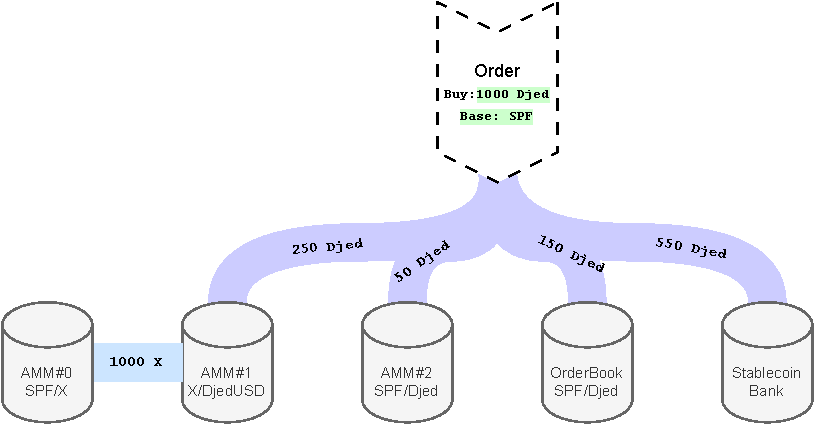
\includegraphics[width=0.98\textwidth]{order_composition}
            \caption{An illustrative example of how one order can be atomically fulfilled from a number of
            different liquidity sources to achieve better price. Some complicated aggregation techniques
            can even involve routing of value through intermediate pools.}
            \label{fig:figure4}
        \end{figure}

        In combination with transparent execution Dutch orders allow to drastically decrease (if not eliminate at all) BEV (MEV) on the platform.

        \newpage


        \section{Autonomous Account: utility in DEXes and beyond}\label{sec:autonomous-account}
        The Autonomous Account primitive can be useful not only in DEXes as we showed previously, but in a much wider range of decentralized applications \
        that can benefit from serving user requests in a non-interactive way without any on-chain overhead.

        We are now showing how AA can be extended to support a dynamic set of applications on eUTxO blockchains that support delegated \
        validation (i.e.\ allows to delegate validation from one script to another).
        Instead of hard-coded logic responsible for validation of a specific request (order), AA now stores just a set of script \
        hashes approved by this account, each hash corresponding to a specific validator that must be \
        evaluated in the case when corresponding application interacts with the account.
        The set of rules can be updated by the user, e.g.\ when a new application needs to be enabled.
        The API of modified AA is described in~\ref{tab:table4}

        \begin{figure}[h!]
            \centering
            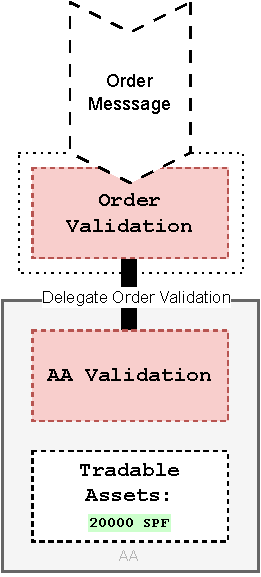
\includegraphics[width=0.25\textwidth]{val_delegation}
            \caption{A modified construction of AA interoperable with an arbitrary number of applications.
            The burden of order validation is now delegated to an external script.}
            \label{fig:figure5}
        \end{figure}

        \newpage
        \appendix
        \section*{Appendix}\label{sec:appendix}

        \begin{table}[h!]
            \begin{center}
                \begin{tabular}{ | r l | }
                    \hline
                    NFT                      & Unique account identifier                        \\
                    $PK_{user}$              & User's public key used for authorization         \\
                    $\{H(V_i) | 0 < i < N\}$ & Set of validator hashes for enabled applications \\
                    \hline
                \end{tabular}
            \end{center}
            \caption{Data structure of AA.}
            \label{tab:table3}
        \end{table}

        \begin{table}[h!]
            \begin{center}
                \begin{tabular}{ | r l | }
                    \hline
                    Order Validation Rules & We omit concrete order validation logic        \\
                    Nonce consistency      & Upon each application of an order require      \\
                    \space                 & that $Nonce_{Ord} = Nonce_{AA}$                \\
                    Nonce increment        & Upon each application of an order require      \\
                    \space                 & that $Nonce_{AA}' = Nonce_{AA} + 1$            \\
                    Valid withdrawal       & Upon receiving a request to withdraw funds     \\
                    \space                 & require that $verify(\sigma, PK_{user}, H(T))$ \\
                    \hline
                \end{tabular}
            \end{center}
            \caption{Structure of AA validation logic. Order Validation Rules may be modular as we point out in Section~\ref{sec:autonomous-account}.}
            \label{tab:table2}
        \end{table}

        \begin{table}[h!]
            \begin{center}
                \begin{tabular}{ | r l | }
                    \hline
                    $ExecRequest(H(V_i))$        & Check that validator with corresponding      \\
                    \space                       & hash $H(V_i)$, where $V_i$ -- i'th supported \\
                    \space                       & validator, is present in the transaction     \\
                    $Deposit(A)$                 & No specific validation is required           \\
                    $Withdraw(A, \sigma)$        & Check that $V' = V - A$, where $V$ -- value  \\
                    \space                       & in AA before withdrawal, $V'$ -- value in AA \\
                    \space                       & after withdrawal.                            \\
                    \space                       & $verify(\sigma, PK_{user}, H(T))$            \\
                    $EnableApp(H(V_i), \sigma)$  & $verify(\sigma, PK_{user}, H(T))$            \\
                    \space                       &                                              \\
                    $DisableApp(H(V_i), \sigma)$ & $verify(\sigma, PK_{user}, H(T))$            \\
                    \hline
                \end{tabular}
            \end{center}
            \caption{API of Autonomous Account.}
            \label{tab:table4}
        \end{table}

        \newpage
        \bibliography{main}
        \bibliographystyle{plain}

    \end{sloppypar}

\end{document}
